\section{Mediciones}

Para las mediciones, creamos listas de compilados de ejemplo de forma aleatoria. Decidimos que el tiempo
de análisis de un compilado fuera un valor aleatorio entre 1 y 99'999, basándonos en los datos de ejemplo
provistos por la cátedra.

Medimos el tiempo de ejecución de nuestro algoritmo para ciertas cantidades de compilados.

Notamos que los procesos de fondo del sistema nos generaba distorciones en los tiempos de ejecución de una misma muestra. Atacamos este problema
realizando varias mediciones para el mismo escenario de compilados y tomando el promedio de los tiempos obtenidos.

Además, como definimos cada escenario arbitrariamente, en una cantidad de compilados $x$, este escenario puede ser poco favorable (puede estar muy desordenado),
mientras que en una cantidad de compilados $x+1$ puede ser muy favorable. Por lo cual la diferencia de tiempos va a ser muy grande a pesar de que la cantidad
de compilados solamente difiere en una unidad (TimSort es una combinación de inserción y mergeSort, por lo cual el desorden inicial toma gran relevancia en el 
rendimiento final del algorítmo). Para solucionar esto, decidimos hacer varios escenarios distintos para la misma cantidad de compilados.

Con el objetivo de comparar los tiempos de ejecución de nuestro algoritmo con la complejidad teórica, optamos por 
realizar tanto un análisis de regresión lineal como uno de regresión lineal logarítmica que se ajustara a nuestros datos.
Para evaluar qué curva se ajusta mejor, usamos la raíz del error cuadrático medio (RMSE). Realizamos este análisis en un
intervalo con tamaños pequeños (hasta 1'000) y en un intervalo con tamaños grandes (hasta 10'000). Ver figuras \ref{fig:tiempos_valores_bajos_puntos} y
\ref{fig:tiempos_valores_altos_puntos}

\begin{figure}[H]
    \centering
    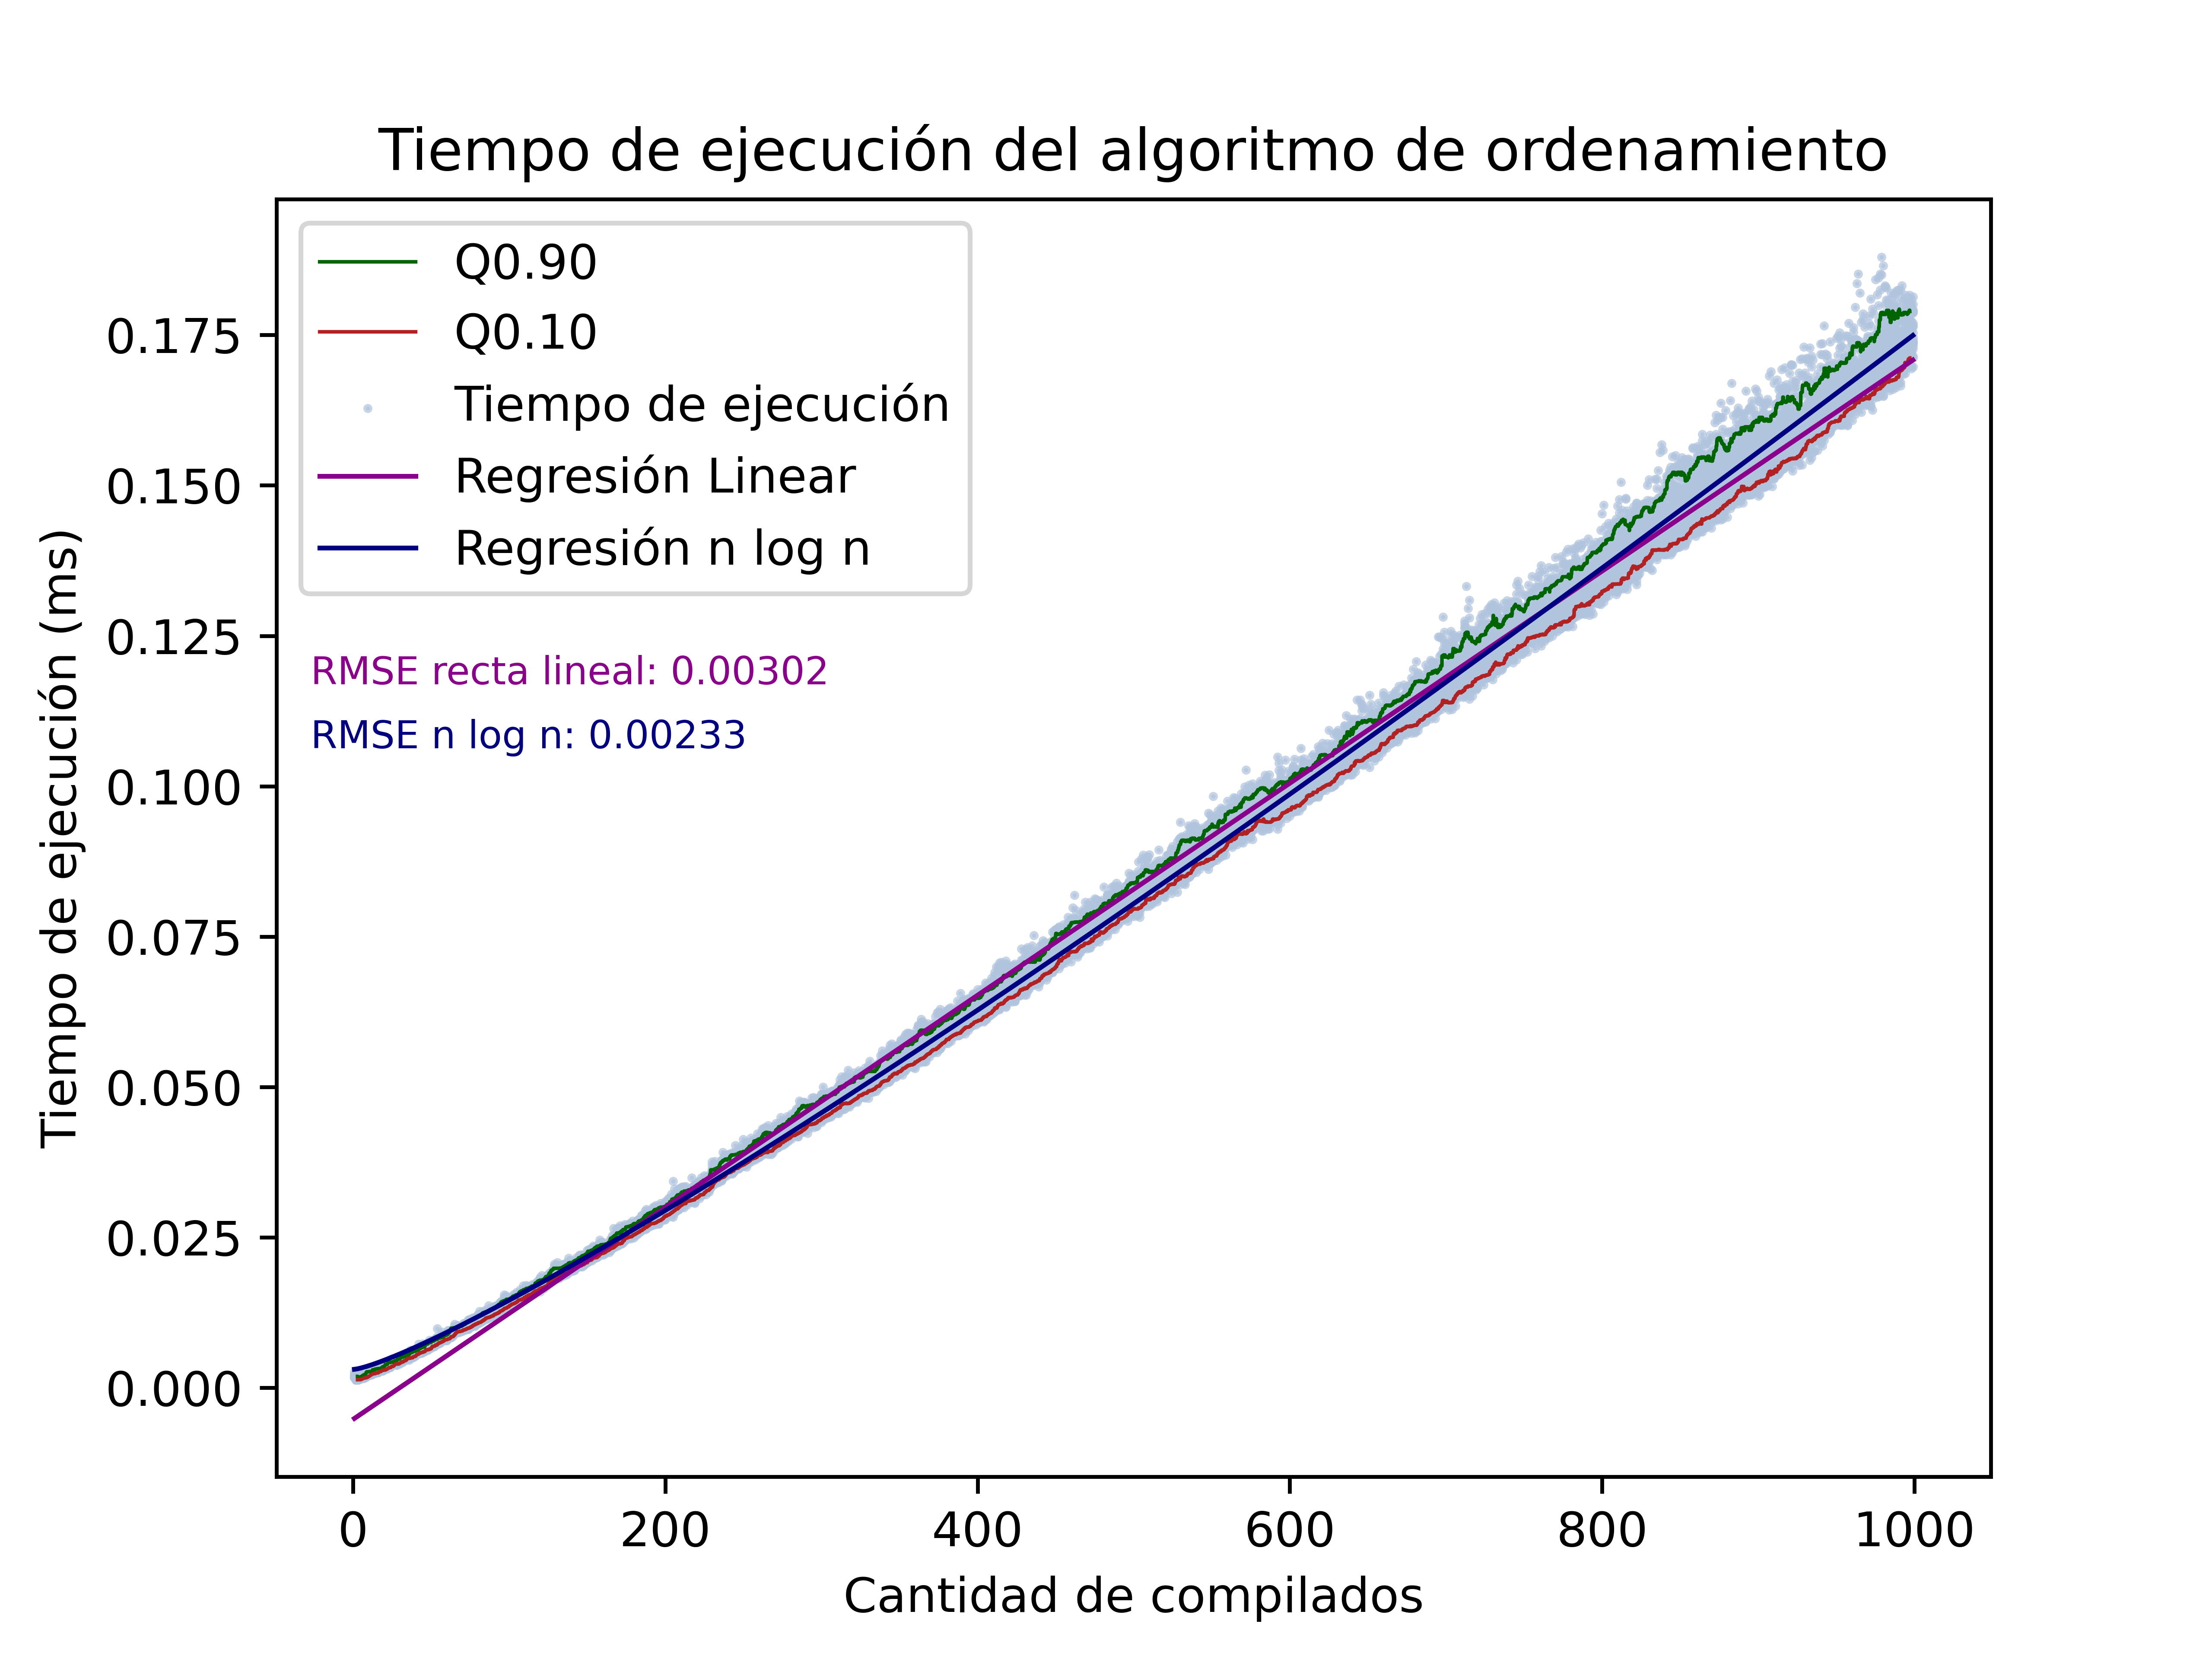
\includegraphics[width=0.8\textwidth]{img/tiempos_valores_bajos_puntos.png}
    \caption{Tendencia de la complejidad algoritmica para $n$ pequeños.}
    \label{fig:tiempos_valores_bajos_puntos}
\end{figure}

\begin{figure}[H]
    \centering
    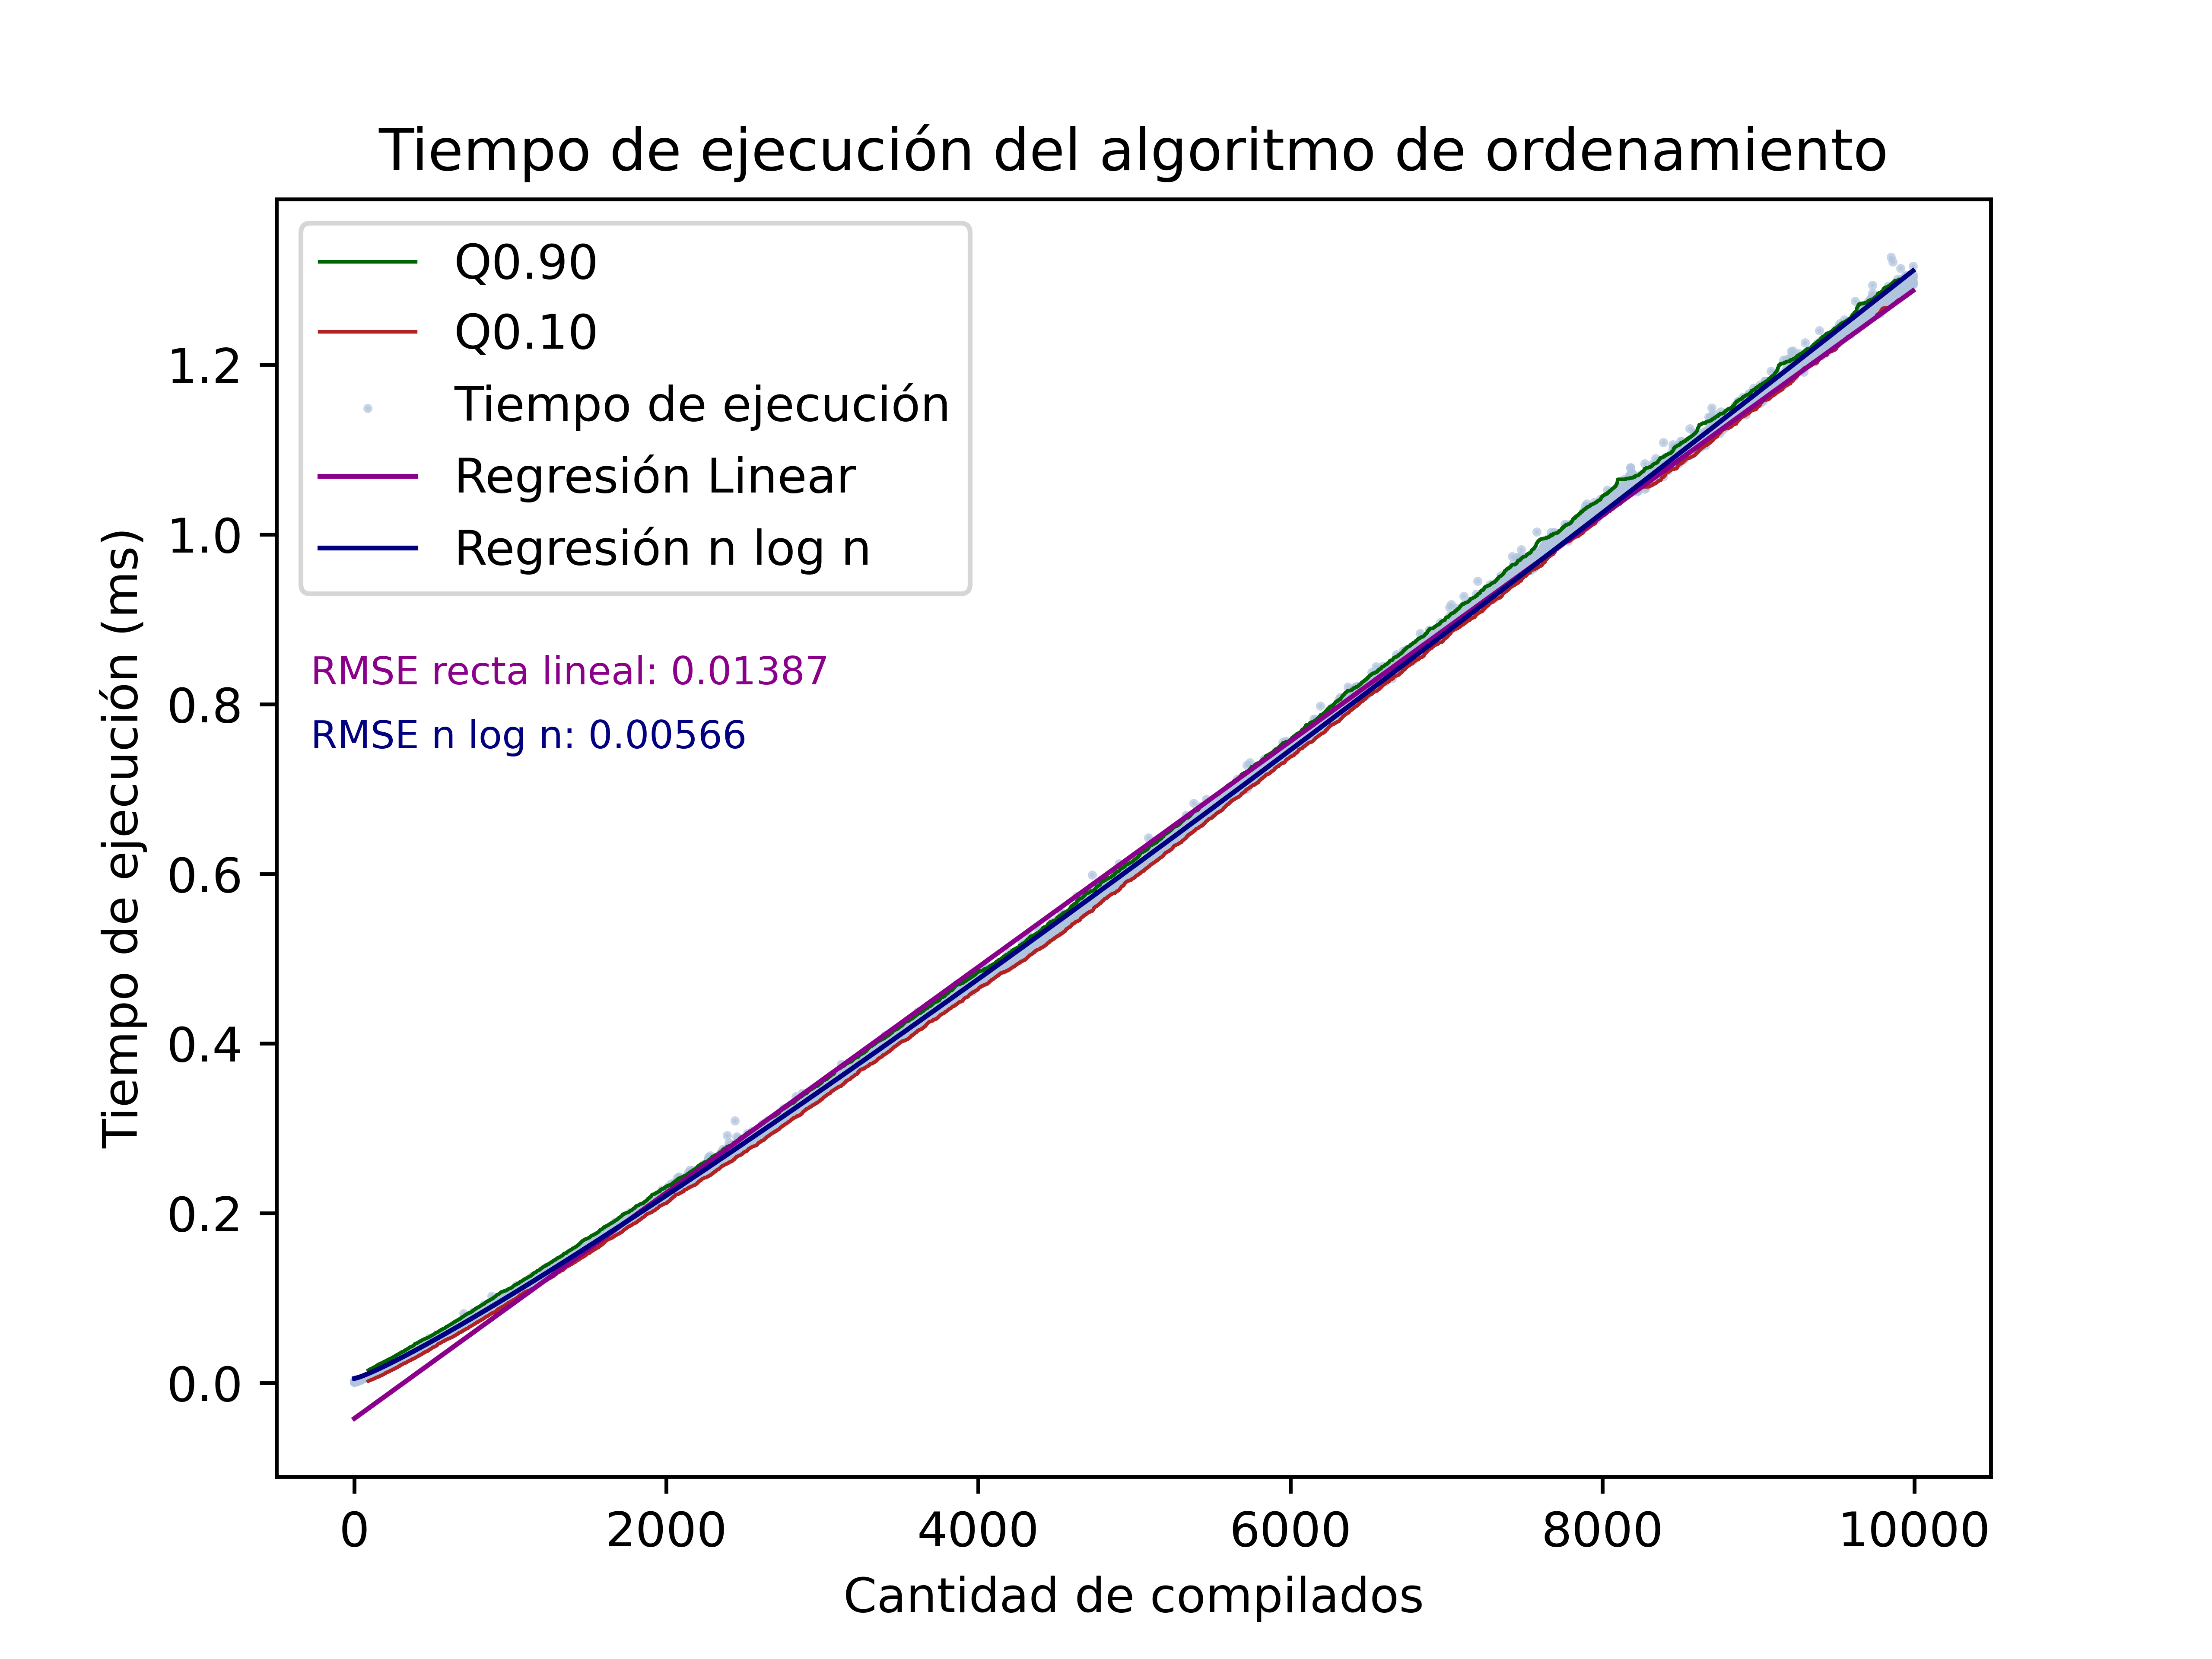
\includegraphics[width=0.8\textwidth]{img/tiempos_valores_altos_puntos.png}
    \caption{Tendencia de la complejidad algoritmica para $n$ grandes.}
    \label{fig:tiempos_valores_altos_puntos}
\end{figure}

Se puede observar que en valores pequeños, el tiempo de ejecución del algoritmo sigue una clara curva lineal logarítmica. Sin embargo, a medida
que aumenta el tamaño de la muestra de compilados, su comportamiento se aproxima más a una complejidad lineal.

Esto ocurre debido a la naturaleza de la función lineal logarítmica, que presenta una pendiente logarítmica. Cuando se 
trabajan con valores grandes, esta pendiente se vuelve casi constante, lo que la asemeja a una función lineal. Esto se 
debe a que el logaritmo es una función monótona creciente, lo que significa que su derivada es siempre positiva para valores 
mayores que cero. Sin embargo, el crecimiento de esta función se vuelve cada vez más lento a medida que los valores aumentan, 
indicando que su segunda derivada es siempre negativa. En consecuencia, para valores muy grandes, la función lineal logarítmica 
se estabiliza y, aunque no es completamente constante, su comportamiento se asemeja a una función lineal.

De esta manera, mediante el gráfico y la validación a través del error cuadrático medio, hemos comprobado que la curva lineal logarítmica 
se adapta de manera más precisa a nuestros datos.

De esta forma pudimos comprobar empíricamente que la complejidad tiende a $\operatorname{O}(n\log{n})$.

Nótese que graficamos también dos curvas que demarcan una estimación de los cuantiles verticales $0.1$ y $0.9$. Esta estimación
se realizó calculando los cuantiles para un grupo pequeño centrado en cada punto. Estas curvas nos ayudan a dimencionar cómo la
varianza del tiempo de ordenamiento crece con el aumento del tamaño de la información de entrada.

Adicionalmente, graficamos la densidad de los tiempos que también brinda una visualización de cómo aumenta la varianza con el aumento del tamaño
de los datos de entrada. Ver figuras \ref{fig:tiempos_valores_bajos_densidad} y \ref{fig:tiempos_valores_altos_densidad} 

\begin{figure}[ht]
    \centering
    \begin{minipage}[b]{0.495\textwidth}
        \centering
        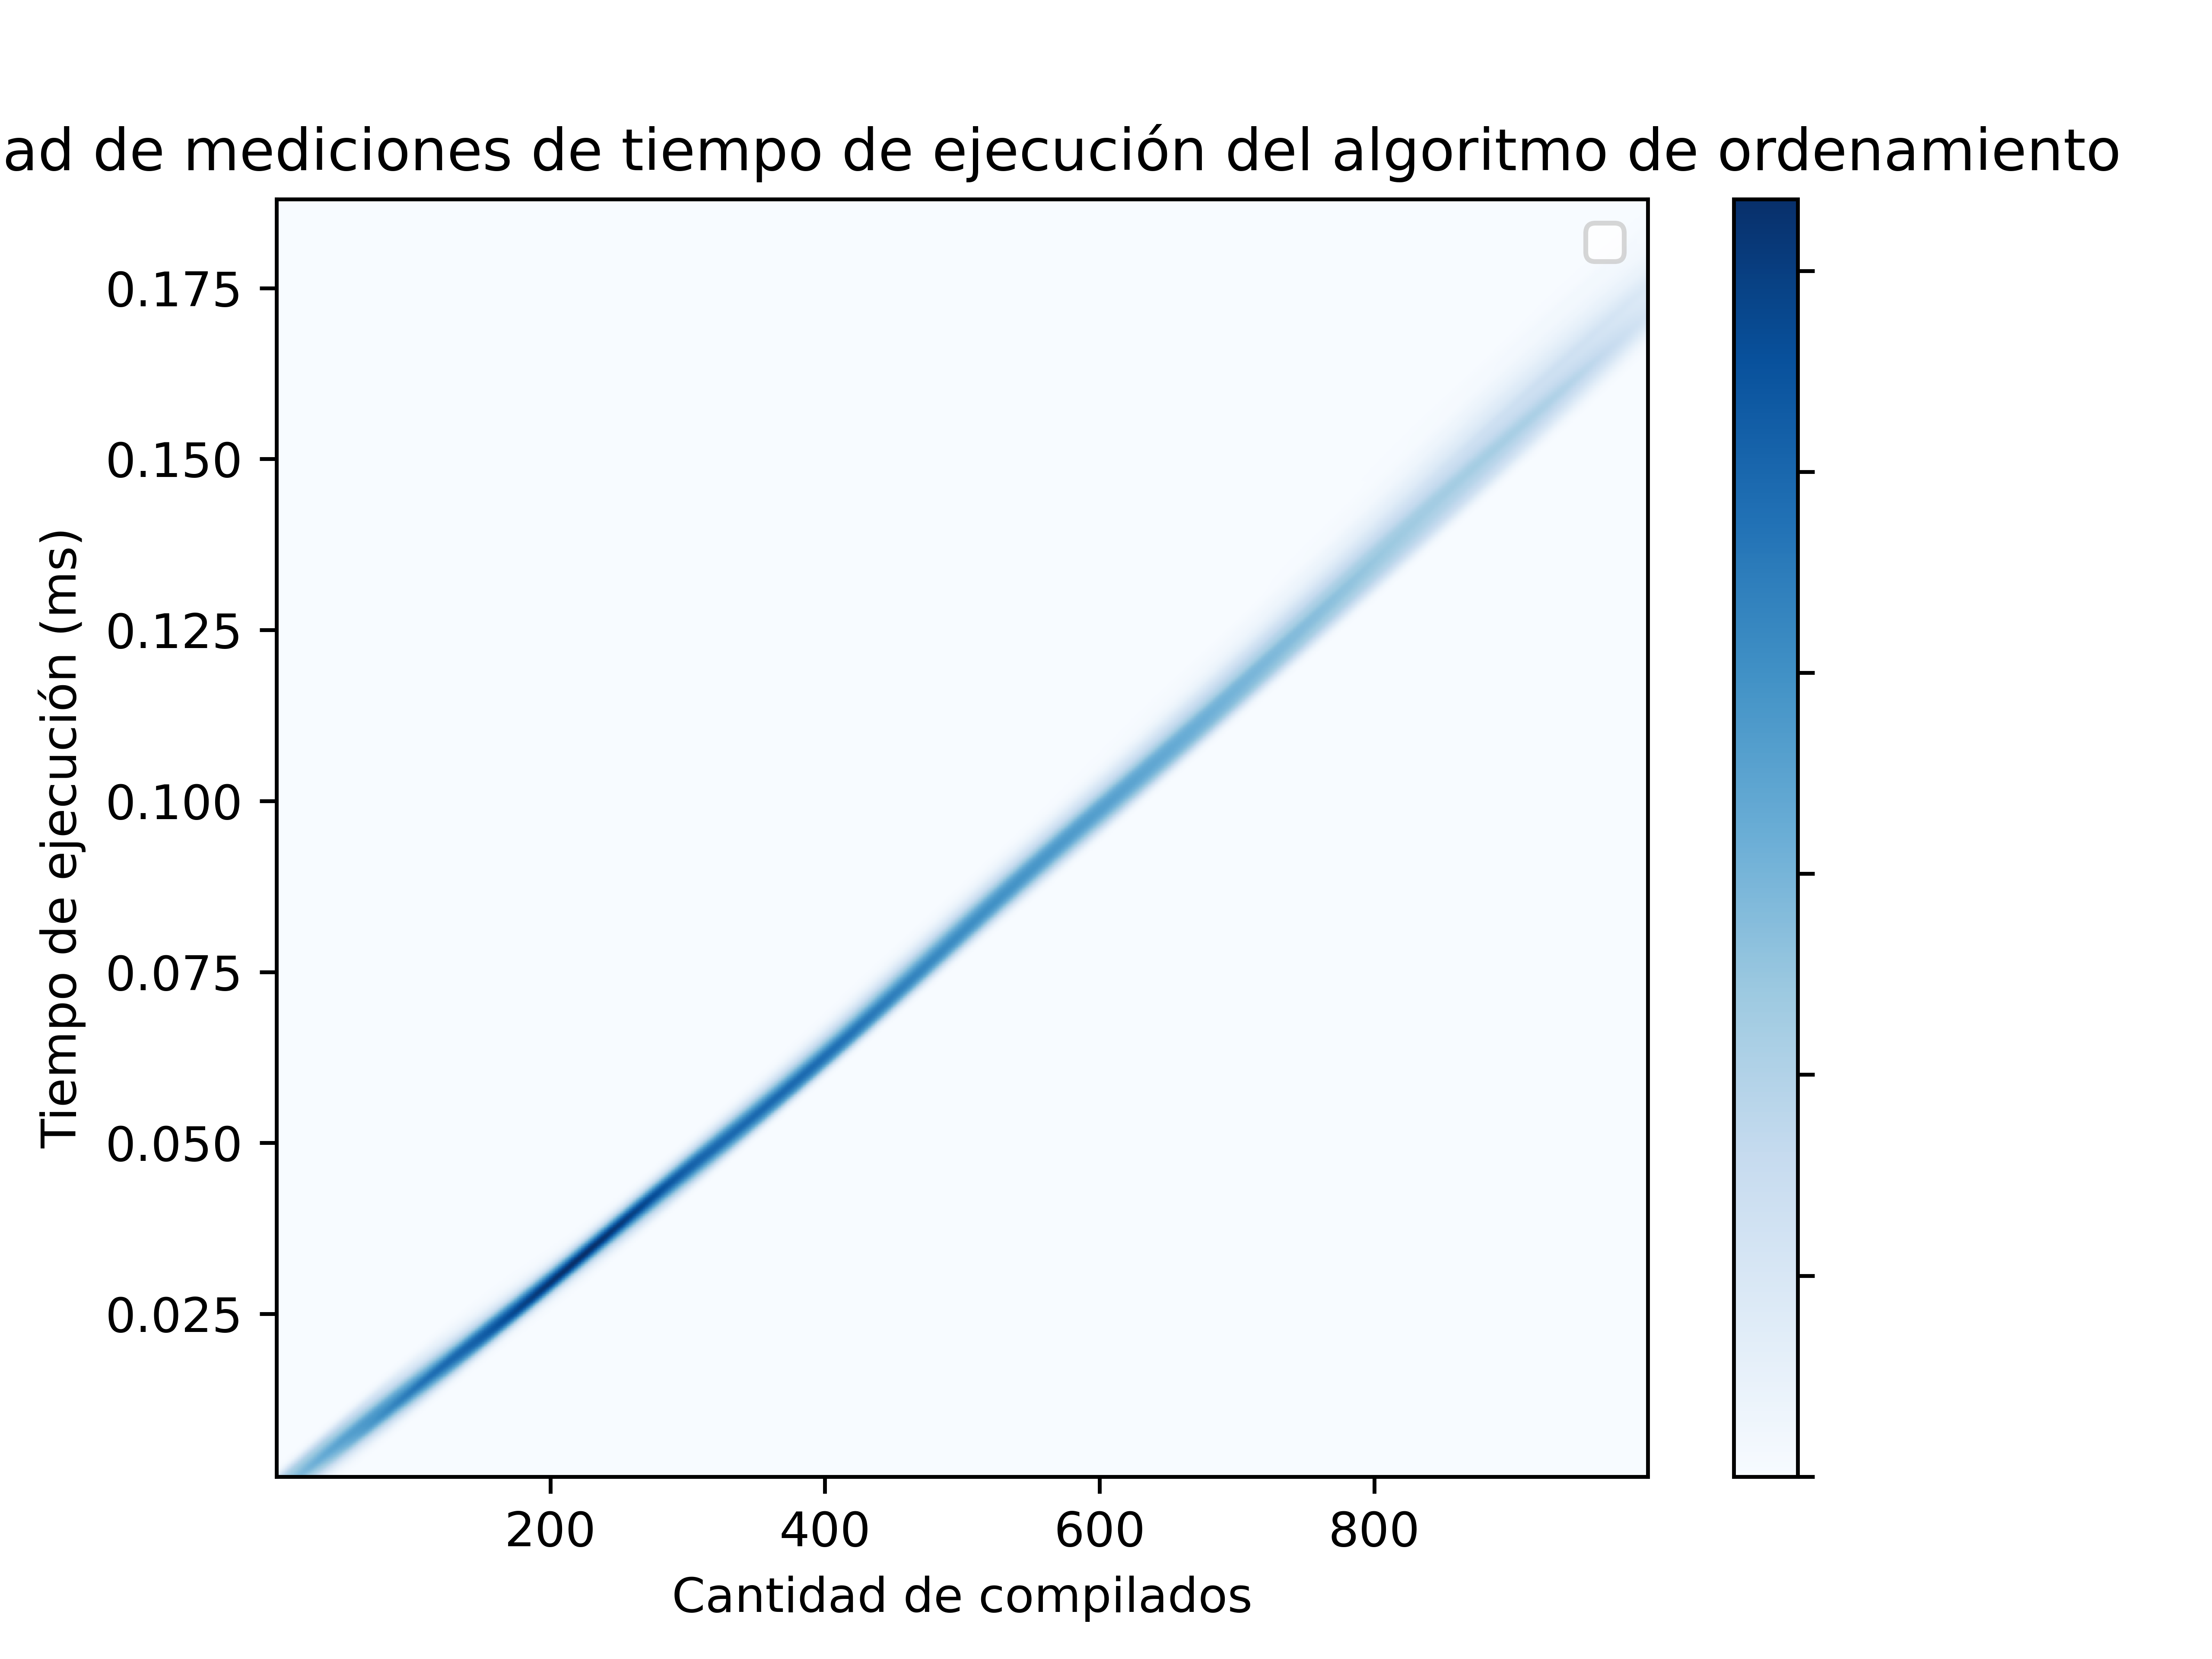
\includegraphics[width=\textwidth]{img/tiempos_valores_bajos_densidad.png}
        \caption{Mediciones para $n$ bajos.}
        \label{fig:tiempos_valores_bajos_densidad}
    \end{minipage}
    \begin{minipage}[b]{0.495\textwidth}
        \centering
        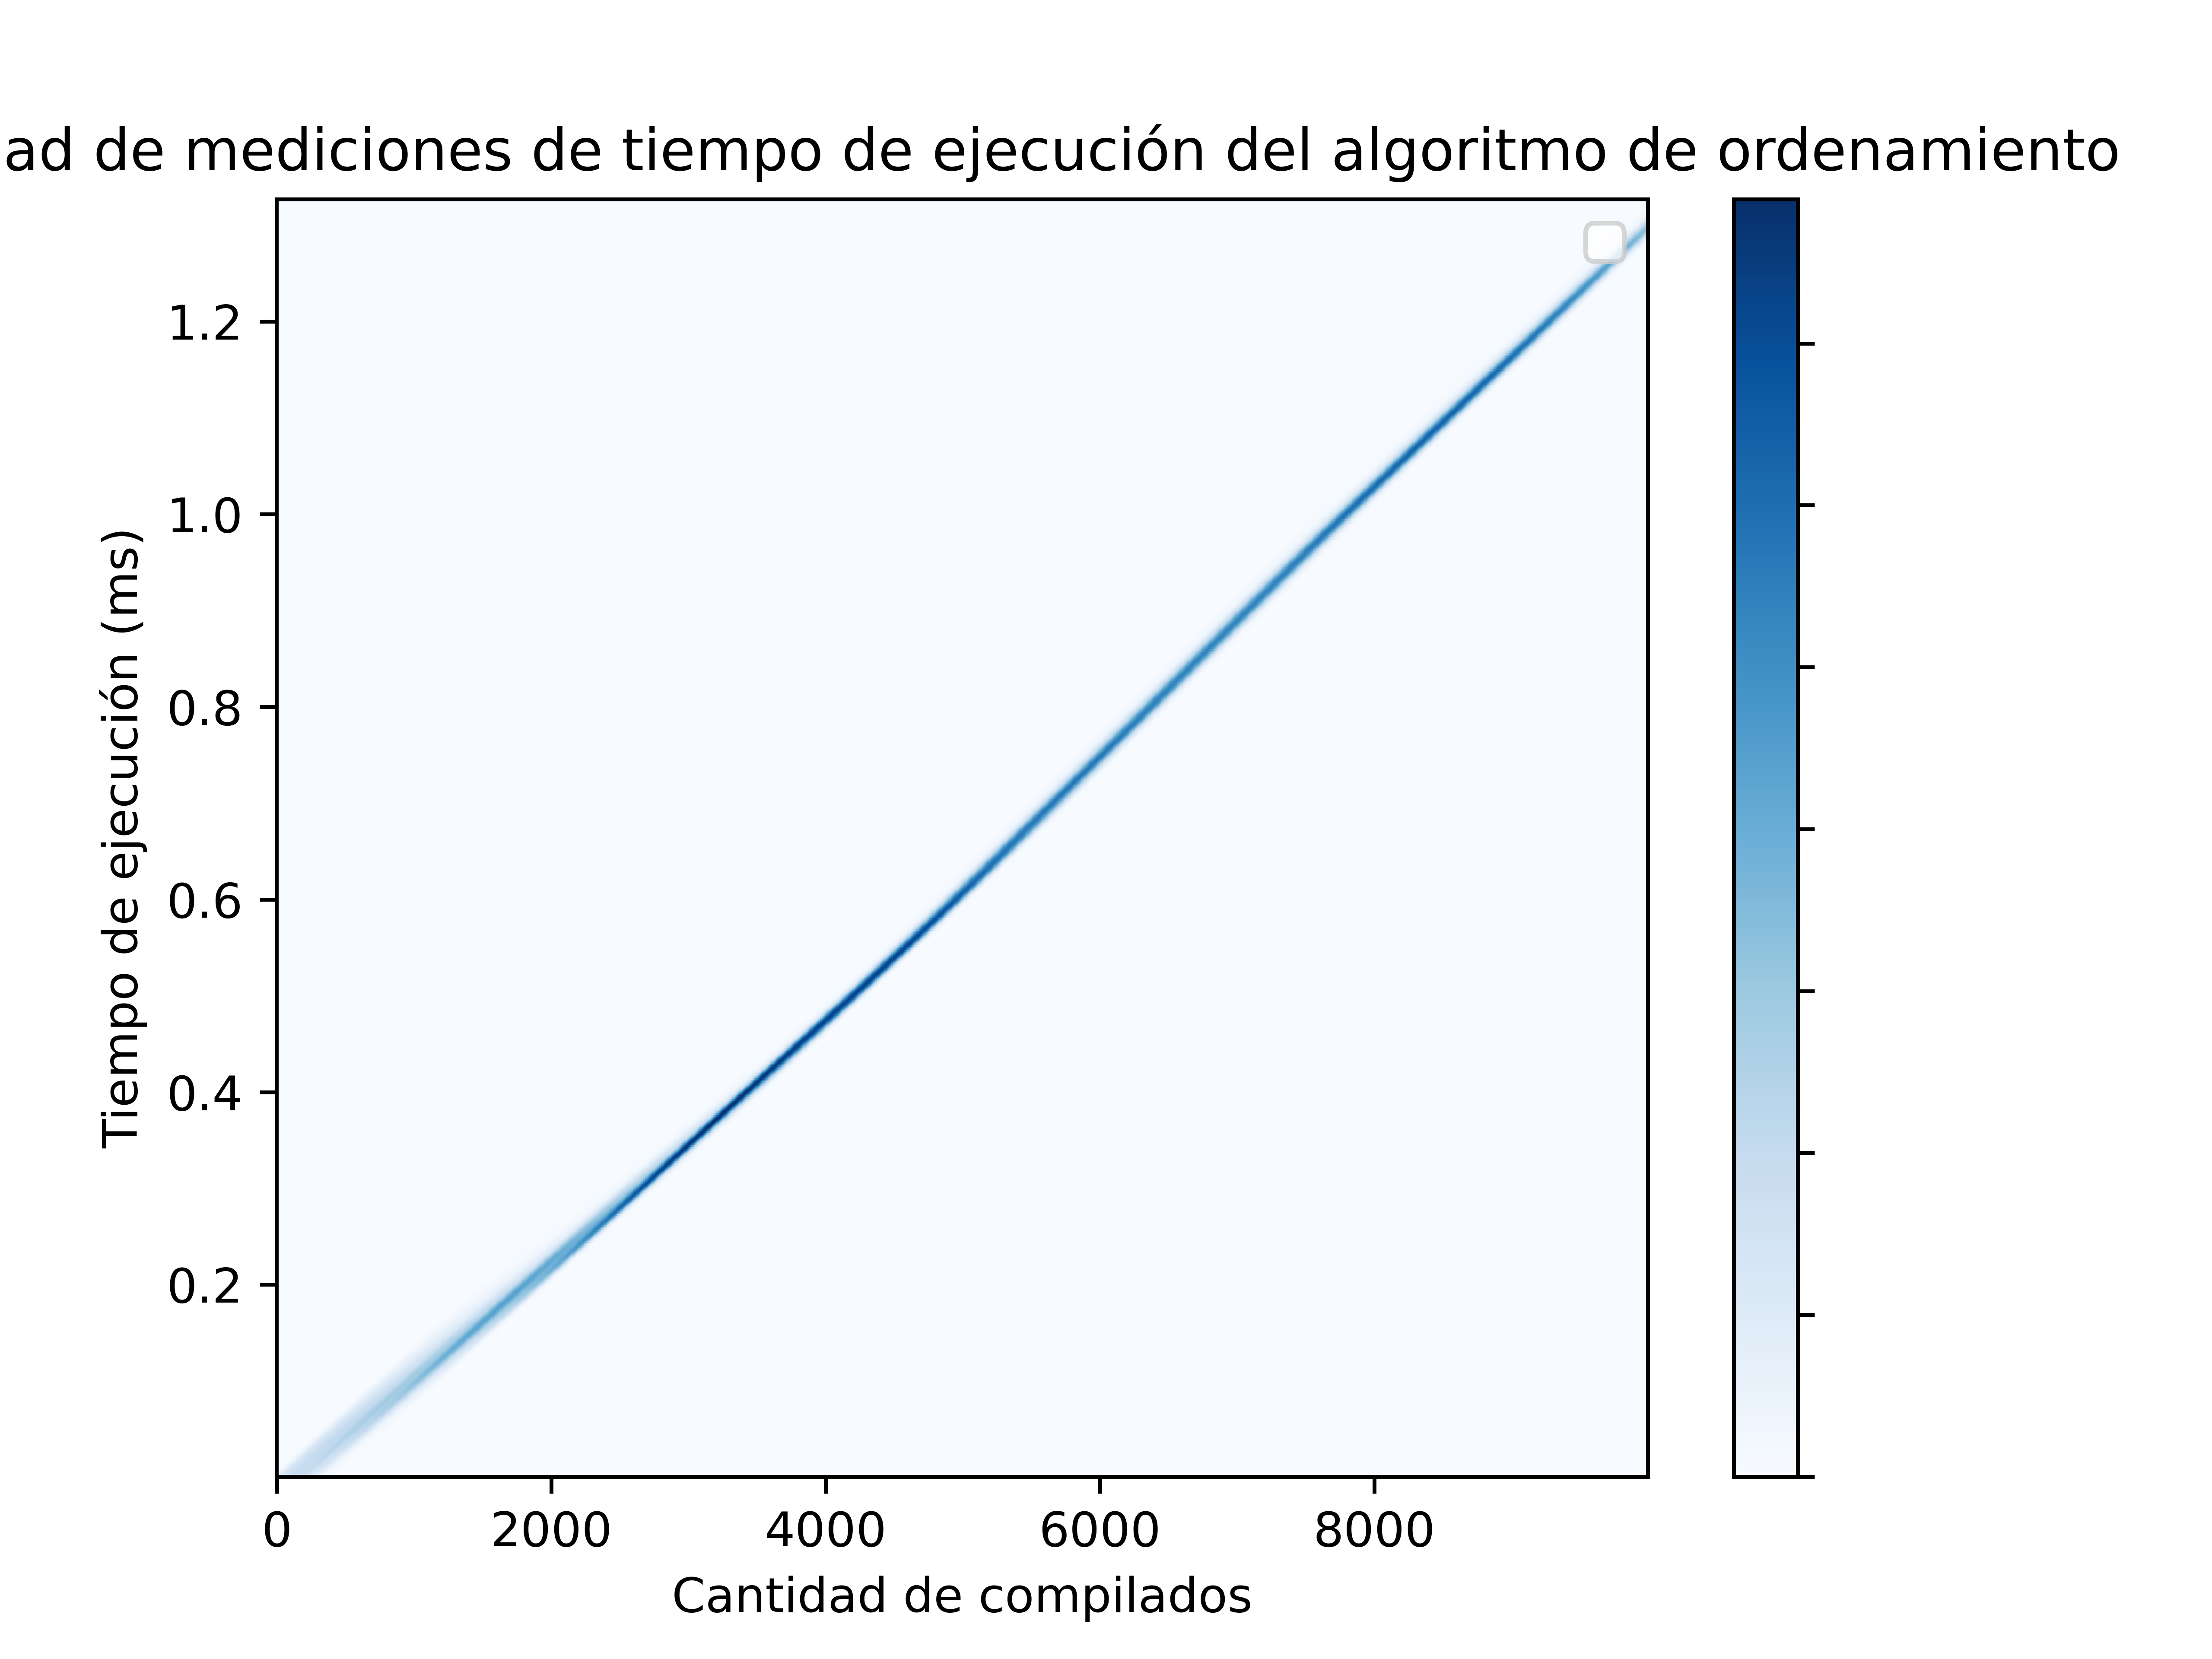
\includegraphics[width=\textwidth]{img/tiempos_valores_altos_densidad.png}
        \caption{Mediciones para $n$ altos.}
        \label{fig:tiempos_valores_altos_densidad}
    \end{minipage}
\end{figure}